\documentclass[11pt,fleqn]{article} 
\usepackage[margin=0.8in, head=0.8in]{geometry} 
\usepackage{amsmath, amssymb, amsthm}
\usepackage{fancyhdr} 
\usepackage{palatino, url, multicol}
\usepackage{graphicx, pgfplots} 
\usepackage[all]{xy}
\usepackage{polynom,tabularx} 
\usepackage{enumerate}
\usepackage{framed}
\usepackage{setspace}
\usepackage{array}
\usepackage{pgf,tikz}
\usepackage{mathrsfs}
\usetikzlibrary{arrows}

\usetikzlibrary{calc}

\pgfplotsset{compat=1.6}

\pgfplotsset{soldot/.style={color=blue,only marks,mark=*}} \pgfplotsset{holdot/.style={color=blue,fill=white,only marks,mark=*}}

\renewcommand{\headrulewidth}{0pt}
\newcommand{\blank}[1]{\rule{#1}{0.75pt}}
\newcommand{\bc}{\begin{center}}
\newcommand{\ec}{\end{center}}
\newcommand{\be}{\begin{enumerate}}
\newcommand{\ee}{\end{enumerate}}

\renewcommand{\d}{\displaystyle}

\usetikzlibrary{calc}
\pgfplotsset{my style/.append style={axis x line=middle, axis y line=
middle, xlabel={$t$}, ylabel={$y$}}}

\pagestyle{fancy} 
%\lfoot{Uses a calculator}
\rfoot{Review: Final Exam (day 1)}

\begin{document}

\vspace*{-0.7in}

\begin{center}
  \large
  \sc{Lecture Notes: Review for Final Exam (day 1)}\\
\end{center}


\bc Summary of Topics \ec
Our final exam will be TUESDAY December 10 from 1:00pm-3:00pm. Jill Faudree's class will be in Chapman 106. Leah Berman's class will be in Duck 342. The Final Exam will be cumulative. You will have 2 hours to complete it. Books, notes, calculators and other aids are not allowed.\\
As with all assessments in this course, you are strongly encouraged to work some old Final Exams as practice.\\

\bc Sample Problems \ec
\begin{enumerate}
\item Given $f(x)= 3x-x^2,$ find $f'(x)$ \emph{using the definition of the derivative.}
\vspace{4in}
\item Find the equation of the line tangent to $ye^x+2=x^2+y^2$ at the point $(0,2).$
\vfill
\newpage
\item Let $F(t)=\frac{20}{4+e^{-2t}}$ model the population of fish in hundreds over time $t$ measured in years. 
\begin{enumerate}
\item Find and interpret $F(0).$
\vfill
\item Find and interpret (in language your parents could understand) $\lim_{t \to \infty} F(t).$
\vfill
\item Find $F'(t).$ (HINT: You can check your answer with the one at the bottom of the page.
\vfill
\item Find and interpret $F'(0).$
\vfill
\item Find and interpret (in language your parents could understand) $\lim_{t \to \infty} F'(t).$
\vfill
\item Give a rough sketch the graph of $F(t)$ given the information above.
\vfill
\end{enumerate}
$F'(t)=\frac{40e^{-2t}}{(4+e^{-2t})^2}$
\newpage
\item Let $f(x)=\frac{5x^2}{1-\cos(x)}.$ 
	\begin{enumerate}
	\item Find  $\d \lim_{x \to 0} \frac{5x^2}{1- \cos x}$
      \vfill
	\item Does $f(x)$ have a vertical asymptote at $x=0$? Explain
	\vfill
	\end{enumerate}
\item Let $g(x)= \frac{4x^4 + 5}{(x^2 - 2)(2x^2 -1)}.$ Does $g(x)$ have any horizontal asymptotes? Justify your answer with a limit.
\vfill


\item Complete two iterations of Newton's Method to estimate a solution to $x^7+4=0$. Use $x_0=-1.$ (Note you may leave your second iteration in unsimplified form.)
\vfill
\newpage
\item Evaluate.
	\begin{enumerate}
	\item $\d \int_0^{\pi/4} \frac{\sec^2 t}{\tan ( t) + 1} dt$
	\vfill
     	 \item $\d \int_0^8 \frac{3}{\sqrt{x+1}} dx$ 
        \vfill
        \end{enumerate}

\item A particle is moving with velocity $v(t) = 2t - \frac{1}{1+t^2}$ measured in meters per second.
	\begin{enumerate}
	\item Find and interpret $v(0).$
	\vspace{1in}
	\item Find the displacement for the particle from time $t=0$ to time $t=4.$ Give units with your answer.
	\vfill
	\item If $D$ is the \emph{distance} the particle traveled over the interval $[0,4],$ is $D$ larger or 	smaller or exactly the same as your answer in part (b)? Justify your answer.
	\vfill
	\item Assuming $s(0) = 1$, find the position of the particle at any time $t$. 
	\vfill
	\end{enumerate}
\end{enumerate}
\end{document}
\newpage

\item The graph of $y = f(t)$
is displayed below. A new function is defined as $H(x)=\int_0^x f(t) \: dt.$\\
 
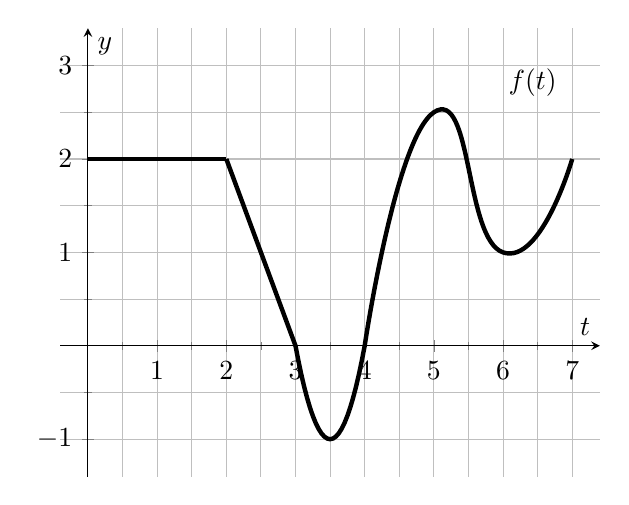
\begin{tikzpicture}
\begin{axis}[scale=1, my style, xtick={0,1,...,7}, ytick={-1,0,...,3},
xmin=-0.4, xmax=7.4, ymin=-1.4, ymax=3.4, 
grid=both, 
%axis equal,
minor y tick num=1, minor x tick num=1, mark size=3.0pt]
\addplot[domain=0:2,ultra thick] {2}; \addplot[domain=2:3,ultra thick]
{6-2*x}; \addplot[domain=3:4,ultra thick] {4*(x-3.5)^2-1};
\addplot[smooth, tension=1, ultra thick] coordinates { (4,0) (5,2.5)
  (6,1) (7,2)};
\end{axis}
\node (o) at (6,5){$f(t)$};
\end{tikzpicture}
\begin{enumerate}
\item Find $f(3).$
\vfill
\item Find $g(3)$
\vfill
\item Find all $x$-values for which $g'(x)=0.$
\vfill
\item Find all $t$-values for which $f'(t)=0.$
\vfill
\item In the open interval $(0,7)$, when does $g(x)$ have a maximum? A minimum?
\vfill
\item When is $g(x)$ increasing?
\vfill
\end{enumerate}
\newpage
\item Find $dy/dx$ for $y=\int_1^{\cos(x)} (1+s^3)e^s \: ds.$
\vspace{2in}
\item A bacteria population is 4000 at time $t = 0$ and
its rate of growth is $1000 \times e^{t/2}$ bacteria per hour after $t$
hours. What is the population after 4 hours? 
\vfill
\item What, if anything, is wrong with the following calculation? 

$$\d \int_0^5 \frac{1}{x-2} dx =  \ln \left( | x- 2 |\right) \Big|_0^5 = \ln (3) - \ln (2)$$
\vspace{1in}

\end{enumerate}
\end{document}






